\documentclass[letterpaper,12pt,oneside]{book}
%\usepackage[a4paper,includeall,bindingoffset=0cm,margin=2cm,marginparsep=0cm,marginparwidth=0cm]{geometry}

    %Paquetes propios de la plantilla
    \usepackage[top=1in, left=0.9in, right=1.25in, bottom=1in]{geometry}
    \usepackage{bachelorstitlepageUNAM}
    \usepackage[utf8]{inputenc}
    
    %Paquetes personales
    \usepackage{fontawesome5}
    
    \usepackage{float}
    \usepackage{graphicx}
    \usepackage[table,xcdraw]{xcolor}
    \usepackage[T1]{fontenc}
    \usepackage[spanish,es-nodecimaldot,es-tabla]{babel}
    \usepackage{tikz} 
    \usepackage{tocloft}
    \usepackage{setspace}
    \usepackage[nottoc]{tocbibind}
    \usepackage[colorlinks,citecolor=red,urlcolor=blue,bookmarks=false,hypertexnames=true]{hyperref} 
    \usepackage{csquotes}
    \usepackage{changepage}
    \usepackage{hyperref}
    
    %Wraping figures----------
    \usepackage{subcaption}
    \usepackage{wrapfig}
    
     \graphicspath{{./figs/}}

    %Comandos personalizados---------
    \newcommand{\figura}[4]{
          \begin{figure}[H]
            \centering
            \includegraphics[scale=#1]{#2}
            \caption{#3}
            \label{#4}
          \end{figure}
                            }
    \newcommand{\refig}[1]{\figurename~\ref{#1}}
    \newcommand{\refeq}[1]{\textbf{ecuación}~\ref{#1}}
    \newcommand{\reteo}[1]{$\mathfrak{Teorema}$~\ref{#1}}
    \newcommand{\bb}[1]{\{#1\}}
    \newcommand{\dd}[2]{ \frac{ #1 }{ #2 } }
    \newcommand{\vals}[2]{ #1$\,$#2 }
    \newcommand{\quotes}[1]{``#1''}
 

    \newtheorem{defi}{\textit{\textmd{$\mathfrak{Definición}$} }}
    \newtheorem{teo}{\textit{\textmd{$\mathscr{Teorema}$} }}


    \renewcommand\cftsecpresnum{\S}
    \renewcommand\cftsubsecpresnum{\S}   

    %Referencias bibliográficas
    \usepackage[ backend=biber,
                 style=apa,
                 uniquename=init,%Requerido para el de abajo
                 minnames=1,
                 maxnames=2,%<----- reduce the number of names on the citation
                 citestyle=authoryear-icomp]{biblatex}
    \addbibresource{bibfile.bib}

%borrar-----------
    \makeatletter
    \let\NAT@parse\undefined
    \makeatother
%borrar-----------
%###################################
% Artículo 12.- El protocolo de tesis, con el visto bueno de un asesor, deberá ser entregado por 
% el alumno a la Coordinación de Carrera correspondiente para su registro, así como para su 
% presentación ante el Comité de Aprobación de Protocolo de Tesis correspondiente. El alumno 
% deberá tener un mínimo del 90% de créditos de su carrera para registrar su protocolo. La 
% Coordinación de Carrera será la responsable de realizar las gestiones académico-administrativas de 
% esta opción de titulación.
% Para someter el protocolo de tesis al Comité de Aprobación de Protocolo de Tesis respectivo, se 
% deberá entregar un documento que no exceda de cinco cuartillas, además de la portada, 
% considerando el contenido siguiente:
%    a) Portada, la cual deberá incluir: título del trabajo de tesis, nombre del alumno y nombre del asesor;
%    b) Objetivo(s) del trabajo;
%    c) Índice tentativo del trabajo de tesis;
%    d) Introducción, antecedentes y justificación del trabajo;
%    e) Metodología a emplear, y
%    f) Bibliografía básica (mínimo 10 referencias)
%###################################

    %Portada------------------------
    \author{Ariel Cerón González}
    %Titulo personal alternativo
    \title{Generación de imágenes con efecto lente gravitacional a partir de pocos ejemplo usando redes generativas antagónicas}
    \faculty{Posgrado en Ciencia e Ingienería de la Computación}
    %\faculty{Instituto de Investigaciones en Matemáticas Aplicadas y en Sistemas}
    \degree{Maestro en Ciencia e Ingeniería de la Computación}
    \supervisor{Dr. Gibran Fuentes Pineda\\ IIMAS, UNAM}
    \cityandyear{CDMX, 2023}
    \logouni{Imagenes/Formales/Escudo-UNAM}
    \logofac{Imagenes/Formales/Escudo-Posgrado}


    \begin{document}    
        %Portada------------------------------
        \frontmatter
        \maketitle
        
        %Oración mamadora--------------------
        \chapter*{}
            \begin{flushright}%
                \vspace*{0.5cm}
                \thispagestyle{empty}
                Machine learning methods implement the scientific principle of “trial and error”.\\

                    \cite{jung2022ml}
            \end{flushright}
            
        %Reumen-----------------------------
        \chapter*{}
        \vspace*{-1.5 cm}
            \begin{center}
                {\LARGE{\bf RESUMEN}}\\
            \end{center}   
                Bajo ciertas condiciones la gravedad genera efectos visuales interesantes. El efecto de {\it lente gravitacional}, descrito por primera vez en la teoría general de la relatividad de Einstein, es un ejemplo. 
                
                Descrito como la alteración espacial realizada por objetos masivos, como colecciones de galaxias, que puede crear campos gravitacionales que distorcionan y magnifican la luz proveniente de galaxias distantes que se encuentran en la misma línea de visión. 

                Existen algunos telescópios, como el Hubble o Euclid, capaces de observar este fenómeno, sin embargo su identificación, y en especial su confirmación, es una tarea difícil lo que explica que a la fecha solo se tenga una centena de datos confirmados.
                
                Las observaciones de este fenómeno pueden ayudar en el estudio de galaxias primitivas, conocer mejor la distribución de las galaxias o buscar exoplanetas que orbiten cerca de grandes soles. 

                Para aumentar la cantidad de elementos se han presentado trabajos que entrenan modelos de clasificación para  ayuden a identificar posibles registros del fenómeno en los datos que los telescopios mencionados han registrado, llegando a tener porcentajes del 88\% de éxito en la identificación.

                El éxito de los modelos de aprendizaje se distribuye en sus componentes principales: los datos, el modelo y la función de pérdida. Cuando alguno de estos elementos tienen deficiencia, el modelo presenta problemas los resultados, un ejemplo es la carencia de datos de calidad, como en el caso del lente gravitacional. 

                Los modelos generativos antagónicos (GAN), por su parte, han sido descritos e implementados de diferentes formas mostrando buenos resultados en la generación de rostros, color de autos o en la identificación de razas de perro; aplicando diferentes condiciones como la poca disponibilidad de datos, diferente calidad de imágenes, poca diversidad en las imágnes, pocos datos de entrenamiento, entre otros.

                Este trabajo se centra en estudiar el problema de la selección de modelo para entrenar modelos GANs con pocos datos que replique el efecto lenticular en nuevos conjuntos de datos, considerando tres estrategías de evaluación 
                \begin{itemize}
                    \item[1.] Cálculo de la métrica FID (Fréchet inception distance) para establecer la calidad en las imágenes generadas. 
                    \item[2.] La puntación F1 con y sin aumentado de datos, del modelo entrenado, usando redes ResNet18 para la identificación de imágenes con efecto lenticular.
                    \item[3.] La revisión de un experto de los experimentos generados.  
                \end{itemize}

                {\bf Palabras clave:} GANs, efecto lenticular, redes profundas.


                
            %{\it Resumen en ingles}\\
                ------------------\\
                \vspace{0.5cm}
                
                \vspace{0.5cm}
                
            
        
        %Dedicatoria-------------------------
        \chapter*{}
            \begin{flushright}%
                \emph{Dedicatoria ...}                        
                \thispagestyle{empty}
            \end{flushright}
            
        %Agradecimientos---------------------
       
        \chapter{Agradecimientos}
             \spacing{1.5}%\doublespacing
                
        %Notación-----------------------------        
       
        \chapter{Notación}
            \begin{itemize}
                \item 
            \end{itemize}

        %Indice--------------------------------
        \newpage
        \tableofcontents
        \newpage
        \listoffigures

        \mainmatter

        %Contenido-----------------------------
       
        \chapter{Introducción}
            La generación de imágenes artificiales es una de las actividades más populares en el campo de la inteligencia artificial, en específico, en el aprendizaje profundo. Muchos de los resultados más realistas son generados con redes generativas antagónicas (GAN). 

            Este trabajo busca utilizar modelos GAN para la generación de imágenes con efecto gravitatorio denominado {\it efecto lenticular}, teniendo como principal reto la cantidad de imágenes disponibles durante el entrenamiento.

            %\section{Antecedentes}

                %\subsection{Redes Generativas Antagónicas}
                \section{Redes Generativas Antagónicas}
                % \begin{wrapfigure}{l}{0.45\textwidth}
                %     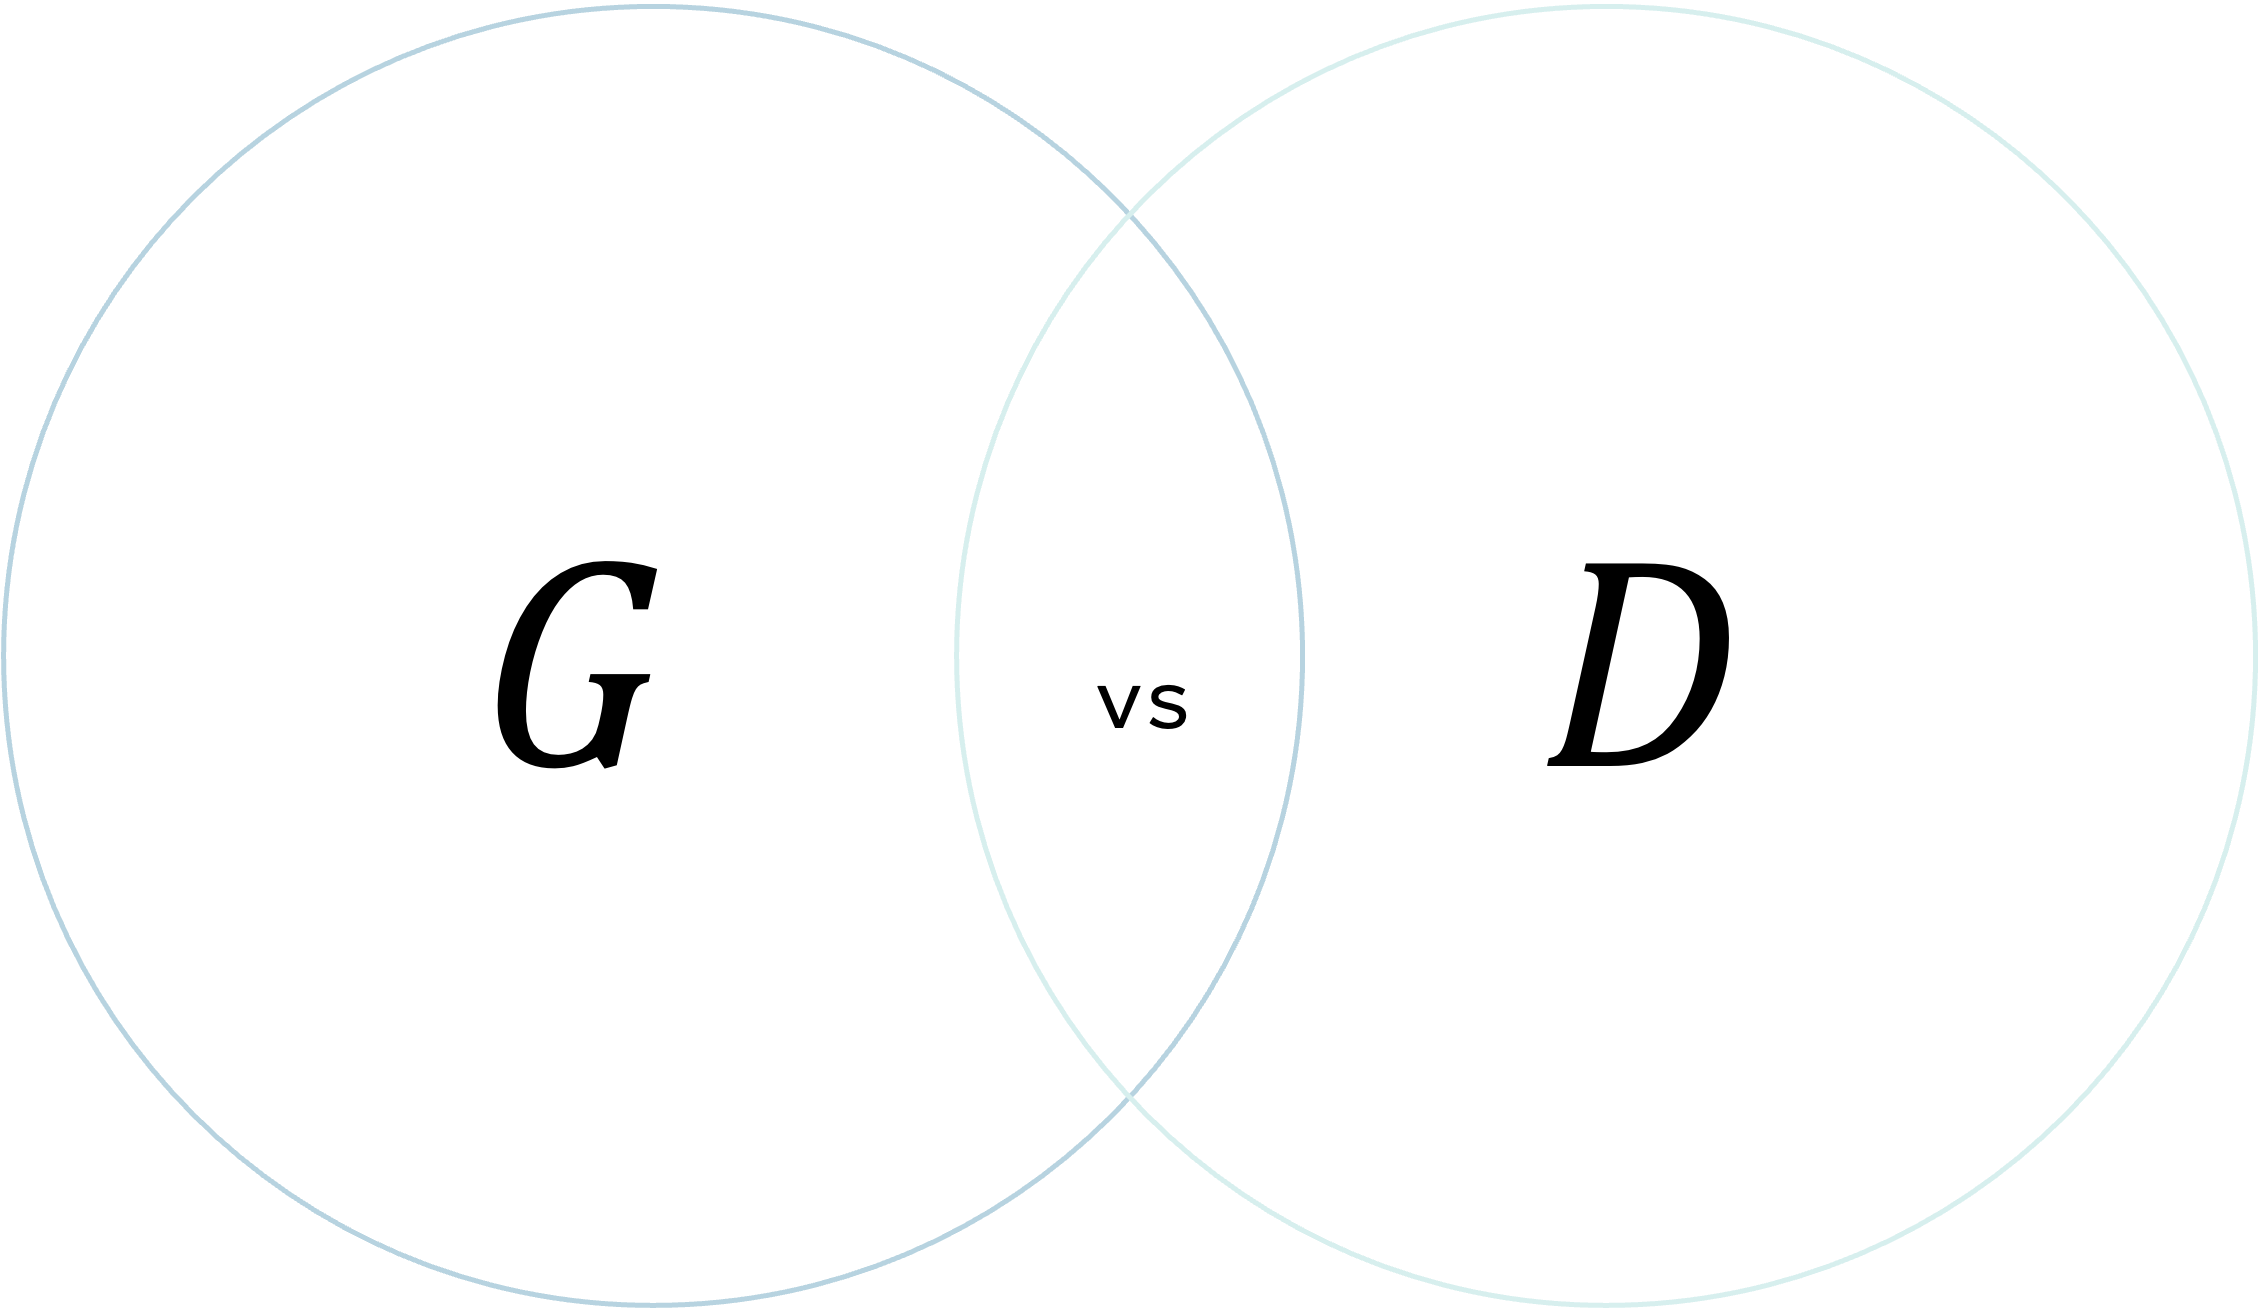
\includegraphics[width=0.9\linewidth]{Imagenes/Resultados/gan_vs.png} 
                %     \caption{La red generadora $G$ se {\it enfrenta} a la red discriminadora $D$ para lograr las mejores configuraciones de cada red.}
                %     \label{fig:gan_vs}
                % \end{wrapfigure}

                \figura{0.45}{Imagenes/Resultados/gan_vs.png}{La red generadora $G$ se {\it enfrenta} a la red discriminadora $D$ para lograr las mejores configuraciones de cada red.}{fig:gan_vs}

                Las GANs son un método (figura \ref{fig:diagrama_gan}) para la optimización competitiva entre dos redes neuronales, una {\it generadora} $G$ y otra {\it discriminadora} $D$, con el objetivo de generar instancias nuevas idealmente indistingibles a las del conjunto objetivo [\cite{de2023redes}].

                Este proceso inicia con un vector $z$, muestreado de una función de probabilidad $p_z$, que alimenta a la red generadora $G$. El objetivo de esta red es lograr que la función $G$ acabe siendo una estimación de la distribución de probabilidad del conjunto de entrenamiento, $G(z) \sim p_g$. Por otro lado, la red discriminadora $D$ toma como entrada imágenes, pueden ser del conjunto objetivo o proveniente de la función generada, el objetivo de esta red es lograr distinguir entre una figura real y una generada.

                Al término del entrenamiento, se espera que la red $G$ {\it gane} el enfrentamiento y sea capaz de engañar a la red discriminadora, aún después de optimizarla. 

                Parte de la popularidad de estos modelos, frente a otros modelos generativos como los VAE (Variational Autoencoders, en inglés), es gracias a la nitidez obtenida en las imágenes, la facilidad para modificar las redes y sus parámetros. 
                    
                    \figura{0.5}{Imagenes/Resultados/diagrama_gan2.png}{Simplificación del proceso de entrenamiento del método GAN.}{fig:diagrama_gan}

                Los modelos GAN han sido desarrollado principalmente para aquellos casos donde los datos son imágenes y dado a que hay diversas implementaciones que pueden cubrir los requerimentos de los datos, como la calidad y falta de datos se vuelven ideales para este texto.
                %Frente a estas ventajas, los modelos han mostrado algunos inconvenientes, como el colapso de la moda, que tiende a genrar un tipo particular de patrón al generar imágenes, el desvanecimiento de gradiente, el cual genera una optimización demasiado rápida e inestabilidad, haciendo que algunos entrenamiento no convergan en un resultado. 

                %\subsection{Lente gravitacional}
                \section{Lente gravitacional}
                    \figura{0.19}{Imagenes/Resultados/space_lens.jpeg}{Figura de un conjunto de galaxias callamod Abell 370 tomada por el telescopio Hubble. Tomada de hubblesite }{fig:space_lens}

                De acuerdo a la relatividad general, la gravedad es una fuerza que distorciona la estructura espacio temporal, ocacionando que objetos como planetas, luz, etc., sufran una curvatura en sus orbitas. En los extremos, la gravedad puede generar efectos visuales interesantes como el de lente gravitacional. 
                
                Un lente gravitacional puede puede ocurrir cuando una gran cantidad de materia, como clusters de galaxias (figura \ref{fig:space_lens}), crean un campo gravitacional que distorciona y magnifica la luz de objetos distantes que se encuentran detrás, pero en la misma línea de visión; una analogía es la de mirar a través de una lupa, lo que permitiría a los investigadores estudiar detalles de galaxias tempranas que se encuentran tan lejos que no pueden ser vistas con la tecnología actual. Además, pueden ser usados para la detección de exoplanetas o el estudio de matería negra. 
                
                Este efecto se clasifica como fuerte, débil y micro. La lente gravitatoria fuerte es capaz de producir múltiples imágenes, como la cruz de Einstein, arcos o anillos y, se cree, que casi cualquier luz de galaxias lejana nos llega afectada por cualquier tipo de lente gravitacional [\cite{khachatryan2021machine}].

                El primer objeto detectado con un lente gravitacional fuerte, diferente al identificado en el eclipse de 1919, ocurrio en 1979 al observsar a un par de quasar y denominado QSO 0957+561. Sin embargo, pese al tiempo desde que se conoce este efecto, las colecciones de imágenes confirmadas con este efecto son menores 1 K elementos. [\cite{khachatryan2021machine}].
            
    
            %\subsection{Generación con pocos datos}
            \section{Antecedentes}
                    \figura{0.25}{Imagenes/Resultados/antecedentes.png}{Conjunto de datos utilizados en otras aplicaciones de aprendizaje profundo. Lado izquierdo usa un modelo generativo de imágenes para entrenar una red calsificadora CNN. Lado derecho, imágenes obtenidas del DESI Legacy Imaging Surveys usando un modelo de clasificación lineal.}{fig:antecedentes}

                La falta de imágenes ha suponido un reto en el entrenamiento de cualquier modelo de aprendizaje máquina [\cite{wilde2022detecting}, \cite{tran2022agel}], algunos autores utilizan modelos numéricos [\cite{vago2022deepgravilens}, \cite{madireddy2019modular}] (figura \ref{fig:antecedentes}) partiendo de parámetros obtenidos de un conjunto de lentes reales, o implementan otro tipo de soluciones. \cite{karras2020training} presenta una estrategía basada en el aumentado de datos ({\it Adaptative Data Augmentation}) la  cual logra estabilizar el entrenamiento con datos limitados, sin alterar la función de perdida o la arquitectura de las redes, además de obtener resultados competitivos, [\cite{wang2018transferring}] por su parte, aprovecha resultados de otros entrenamientos, buscando afinar el entrenamiento hacía el nuevo dominio de interes, presentando resultados de buena calidad en menos iteraciones. 


            Tenemos la hipótesis de que si se utiliza el aumentado de datos y la transferencia de conocimiento en un modelo GAN entonces se podría entrenar con los elementos existentes y obtener una red generadora $G$ con resultados competitivos que aproxime el lente gravitacional. 

            Este trabajo tiene como objetivo trabajar con diferentes arquitecturas GANs, medir la calidad de los resultados con pocos datos y después pasarlas por una combinación de aumentado de datos y transferencia de conocimiento. Los resultados serán comparados para mostrar las ventajas de esta implementación con tres formas diferentes para medir los resultados:


            \begin{itemize}
                \item[1.]Evaluar los resultados de diversas arquitecturas GAN, aplicando algunos métodos que reduzcan el costo computacional, el colapso de la moda, no sea necesario el uso de grandes conjuntos de datos y que acepten transferencia de conocimiento
                \item[2] Evaluación de los resultados en tres formas 1) con la ayuda de un experto, que visualmente confirme la afinidad de las imágenes generadas con las que puedan existir en la realidad, 2) usando FID para la evaluación de las imágenes generadas y 3) entrenando un modelo de clasificación que pueda reconocer imágenes reales de galaxia con efecto lenticular.  
            \end{itemize}
            
            


            
            
        \chapter{Desarrollo}
            El desarrollo de nuevos objetos digitales para estudios astronómicos ha incrementado el tamaño y la compejidad de los datos recolectados. Siendo que la identificación de objetos {\it raros} sea escencial para facilitar ciertos estudios, el uso de nuevas herramientas para su identificación se vuelve una tarea necesaria. Para dar un ejemplo, el lanzamiento del conjunto de datos del 2019 del {\it Dark Energy Spectorscopic Instrument (DESI) Legacy Imaging Surveys}, incluye $\mathcal{O}(10^9)$ galaxias, un número que deja fuera a la detección manual. 


            % Los elementos principales de un modelo de aprendizaje son: 1) un conjunto de datos, 2) un conjunto de hipótesis y 3) una función de perdida [\cite{prince2023understanding}]. 

            \section{DESI Legacy Survey}
                Los lentes gravitacionales fuertes pueden presentarse en diferentes configuraciones visuales, incluyendo la parición de entornos y vecinos similares y la identiicación de un lente gravitacional mediante inspección visual puede ser una actividad complicada. 

                Después de una extracción de candidatos de diferentes fuentes como: {\it The Master Lens Database}, tablas pubicadas a través de VizieR database y {\it The Survey of Gravitationally-lensed Objects} \cite{stein2022mining} pone a disposición un catálogo, con 1192 muestras, verificadas y usadas en el mismo artículo como conjunto de entrenamiento, y validación, a un modelo de aprendizaje no supervisado. 

                \figura{0.35}{Imagenes/Resultados/training_lenses}{Sesenta y nueve ejemplos aleatorios del efecto gravitacional fuerte, del conjunto de datos denominado entrenamiento.}{fig:desilegacy}


                \subsection{Catálogo de datos}
                    %Los rayos de luz son reflectados cuando se propagan a través de un campo gravitacional no homogeneo y aunque muchos investigadores tuvieron diferentes especulaciones acerca de este efecto, no fue sino hasta después de la presentación de la teoría general de la relatividad que se tuvo una hipótesis certera. [\cite{bermano2022state}]
                    Los resultados obtenidos por \cite{stein2022mining} se encuentran en un proyecto de acceso público alojado en \href{https://github.com/georgestein/ssl-legacysurvey/tree/main/strong_lensing_paper}{Github}; estos recopilan, después de un proceso de inado de información, diferentes ejemplos del efecto lenticular fuerte confirmados por la comunidad, además presenta un conjunto extra de imágenes detectados después de aplicar un algoritmo de clasificación.

                    El {\it DESI Legacy Imaging Surveys} cubre aproximadamente 19, 721 grados cuadrados de cielo extragalactico visible desel el hemisferio norte en trs bandas ópticas (g, r, z). Las observaciones (figura \ref{fig:desilegacy}) provienen del último lanzamiento mostrado en la \href{https://www.legacysurvey.org/dr9/description/}{página principal} lanzada en enero de 2021.

                    Desde el portal del {\it National Energy Research Scientific Computing Center} se puede acceder a un portal web que alberga los diferentes archivos utilizados en \cite{stein2022mining}. En este trabajo se obtuvieron cuatro archivos, dos en formato tvs, que obtiene informació en forma de tabla de las coordenadas de los diferentes elementos espaciales que después pueden ser obtenidos desde el portal del DESI haciendo una consulta con las coordenadas. También ofrecen los archivos en un formato H5py, el cual confiere ventajas al momento de hacer la manipulación de grandes volúmenes de datos. 

                        \figura{0.55}{Imagenes/Resultados/flujo_datos}{Adquisición de datos por dos rutas, la primera obtiene los archivos del portal DESI utilizando las coordenadas contenidas en los archivos {\it tsv}. En la segunda ruta, los archivos se encuentran almacenados en formato HDF5.}{fig:flujo_datos}
                
                \subsection{FastGAN}
                
        

            \section{Un conjunto de hipótesis}
                De forma general, se define como hipótesis a una familia de funciones que intentan, de alguna forma, aprender alguna caracteristica del conjunto de datos $\mathcal{D}$. 

                Nuestro escrito tiene como hipótesis principal al modelo conocido como {\bf red generativa adversaria }o GAN por sus siglas en ingles, {\it generative adversarial network} es un modelo no supervisado cuyo objetivo es el de generar nuevos ejemplos indistinguibles, a partirr de un conjunto de ejemplos de entraniento.
                
                \figura{0.25}{Imagenes/Resultados/gan_arc}{Arquitectura básica de un modelo GAN. Un vector ${\bf z}$ dek espacio latente pasa a través del modelo generador $g$ para crear un ejemplo ${\bf x^*}$. Se genera un conjunto de imágenes falsas $\bb{{\bf x^*}}$ e imágenes reales $\bb{{\bf x}}$ que pasan por el modelo discriminador $f$. Por último se modifican los parámetros de cada modelo y se repite el funcionamiento hasta que se llegue a una convergencia de Nash. [\cite{prince2023understanding}]}{fig:gan_arc}

                En 2014 se presenta {\it Generative Adversarial Net} el cual propone una arquitectura para la estimación de modelos generativos vía un entrenamiento adversario. 
                La arquitectura GAN se compone de dos modelos de redes neuronales, uno denominado generador, $G = [{\it z_j}, \theta]$ con ${\bf z_j}$ un vector del espacio latente y $\theta$ el conjunto de parámetros del modelo, cuyo encargo es el de generar nuevas instancias del mismo dominio que del conjunto de datos de origen, y un discriminador $D[{\bf x}, \phi]$ con $x$ un ejemplo y $\phi$ el conjunto de paráemtros del modelo, discrimina si los datos de entrada provienen el del dominio de datos de origen o si son imágenes del generador. Ambas redes se entrenan de manera conjunta, de manera que $G$ maximice sus posibilidades de no ser detectadas por $D$ y $D$ minimice la cantidad de malas detecciones. Estas dos redes antagónicas compiten en un juego de suma cero en el que se hipotetiza que eventualmente llegan a un equilibrio de Nash.

                \subsection{Mode dropping}
                    Los modelos GANs son modelos relativamente sencillos que transforman ruido aleatorio en datos indistinguibles a un conjunto de entrenamiento. Sin embargo, los modelos GAN originales presentan diferentes problemas durante el entrenamiento y después. 

                    Un problema común del modelo es cuando genera ejemplos plausibes pero solo representan un subconjunto específico de los datos, por ejemplo si el modelo esta generando rostros y ocurre este problema, puede que no genere nunca imágenes con barba. Una versión extrema de este problema ocurre cuando el modelo ignora por completo el vector latente ${\bf z}$ y colapsa a un conjunto específico de ejemplos, este probelma se conoce como colapso de la moda (mode collapse).

                    Esto ocurre por la definición propuesta en el modelo GAN original 
                    
                    \begin{eqnarray}
                        \label{eq:loss_gan_origin}
                        L[\phi] &=& \sum -\log[1 - sig[D[G[{\bf z_j, \theta}],\phi]]] - \sum \log[sig[D[{\bf x_i}, \phi]]]\\
                        L[\theta] &=& \sum log[1 - sig[D[G[{\bf z_j}, \phi]]]]
                    \end{eqnarray}

                    Esta función penaliza regiones con ejemplos reales pero no muestras, lo que fuerza a una convergencia. Si nos fijamos en la ecuación \ref{eq:loss_gan_origin} podemos observar que el segundo término de la primera ecuación no depende del generador, por concecuencia no le interesa la convergencia. Lo que a su vez genera el problema de {\it mode dropping}.

                    Una mejora sustancial al modelo ocurre al modificar la función de perdida. Muchos modelos GAN usan la función de perdida conocida como Wassertein. La cula funciona aún cuando las distribuciones son disjuntas y decrecen de forma lenta. 

                    

                \subsection{Deep convolutional GAN}

                    %Aquí agregar un resumen de los problemas de este modelo y cómo se han ido satisfaciendo las necesadidades haciendo modificaciones en las funciones de perdida, los optimizadores, las matodologías y las arquitecturas, para intoduci a los modelos con los que estamos trabajando 
                    
                \subsection{FastGAN}

                \subsection{styleGAN}

            
            


        \printbibliography
        \nocite{*}
        \backmatter%@sglvgdor

    \end{document}


